\documentclass[12pt]{article}%
\usepackage{amsfonts}
\usepackage{fancyhdr}
\usepackage{comment}
\usepackage[a4paper, top=2.5cm, bottom=2.5cm, left=2.2cm, right=2.2cm]%
{geometry}
\usepackage{times}
\usepackage{amsmath}
\usepackage{changepage}
\usepackage{amssymb}
\usepackage{appendix} 
\usepackage{graphicx}%
\usepackage{epstopdf}
\setcounter{MaxMatrixCols}{30}
\newtheorem{theorem}{Theorem}
\newtheorem{acknowledgement}[theorem]{Acknowledgement}
\newtheorem{algorithm}[theorem]{Algorithm}
\newtheorem{axiom}{Axiom}
\newtheorem{case}[theorem]{Case}
\newtheorem{claim}[theorem]{Claim}
\newtheorem{conclusion}[theorem]{Conclusion}
\newtheorem{condition}[theorem]{Condition}
\newtheorem{conjecture}[theorem]{Conjecture}
\newtheorem{corollary}[theorem]{Corollary}
\newtheorem{criterion}[theorem]{Criterion}
\newtheorem{definition}[theorem]{Definition}
\newtheorem{example}[theorem]{Example}
\newtheorem{exercise}[theorem]{Exercise}
\newtheorem{lemma}[theorem]{Lemma}
\usepackage{listings} 
\lstset{language=Matlab}
\lstset{breaklines}
\newtheorem{notation}[theorem]{Notation}
\newtheorem{problem}[theorem]{Problem}
\newtheorem{proposition}[theorem]{Proposition}
\newtheorem{remark}[theorem]{Remark}
\newtheorem{solution}[theorem]{Solution}
\newtheorem{summary}[theorem]{Summary}
\newenvironment{proof}[1][Proof]{\textbf{#1.} }{\ \rule{0.5em}{0.5em}}

\newcommand{\Q}{\mathbb{Q}}
\newcommand{\R}{\mathbb{R}}
\newcommand{\C}{\mathbb{C}}
\newcommand{\Z}{\mathbb{Z}}

\begin{document}

\title{Homework}
\author{Jingcheng Lu [42326170], Yunpeng Hu [13606024]}
\date{\today}
\maketitle
\section{Task1}
\subsection{Euler method}
First, we assume the mass is 1(same for below questions), then we can get the following equation:
\[\begin{array}{l}
{x_{i + 1}} = {x_i} + h{v_i}\\
{v_i} = {v_{i - 1}} + h{a_{i - 1}}\\
{a_{i - 1}} = {{x''}_{i - 1}} =  - {x_{i - 1}}\\
\end{array}\]
Also we know:
\[\begin{array}{l}
{v_{i - 1}} = {{x'}_{i - 1}}\\
{x_{i + 1}} = {x_i} + h \cdot ({v_{i - 1}} + h{a_{i - 1}})\\
 = {x_i} + h \cdot ({{x'}_{i - 1}} - h \cdot {x_{i - 1}})\\
 = {x_i} + h \cdot {{x'}_{i - 1}} - {h^2} \cdot {x_{i - 1}})
\end{array}\]
So, we can conclude that:
\[{x_{i + 1}} = x({t_i}) + h \cdot x'({t_{i - 1}}) - {h^2} \cdot x({t_{i - 1}}))\]

Applying Taylor expansion for \(x({t_{i + 1}})\) at \({t_{i}}\), we can get:

\[\begin{array}{l}
x({t_{i + 1}}) = x({t_i}) + h \cdot x'({t_i}) + \frac{{{h^2}}}{{2!}}x''({t_i}) + O({h^3})\\
x({t_{i + 1}}) - {x_{i + 1}} = h(x'({t_i}) - x'({t_{i - 1}})) + \frac{{{h^2}}}{2}x''({t_i}) + {h^2}x({t_{i - 1}}) + O({h^3})
\end{array}\]

Applying Taylor expansion for \(x'({t_{i}})\) at \({t_{i-1}}\), we can get:
\[x'({t_i}) = x'({t_{i - 1}}) + h \cdot x''({t_{i - 1}}) + O({h^2})\]
Then we applying above equation:
\[\begin{array}{l}
x({t_{i + 1}}) - {x_{i + 1}} = h(h \cdot x''({t_{i - 1}}) + O({h^2})) + \frac{{{h^2}}}{2}x''({t_i}) + {h^2}x({t_{i - 1}}) + O({h^3})\\
 = {h^2}(x''({t_{i - 1}}) + \frac{1}{2}x''({t_i}) + x({t_{i - 1}})) + O({h^3}) = O({h^2})
\end{array}\]
So the error of Euler method is \(O({h^2})\). Thus the global error is \(O({h})\).
\\
The picture \ref{euler1} shown below is the result of Euler method.
\\
As we can see in the picture, the slope is 1, so again it proves our conclusion that Euler method is 1st order.


\subsection{Leapfrog method}
First, we can get:
\[\begin{array}{l}
{x_{i + 1}} = {x_i} + h{v_{i + 0.5}}\\
{v_{i + 0.5}} = {v_{i - 0.5}} + h{a_i}
\end{array}\]
so:
\[\begin{array}{l}
{x_{i + 1}} = {x_i} + h \cdot ({v_{i - 0.5}} + h{a_i})\\
 = {x_i} + h \cdot x'({t_{i - 0.5}}) + {h^2} \cdot x''({t_{i - 0.5}})
\end{array}\]

Applying Taylor expansion for \(x({t_{i + 1}})\) at \({t_{i}}\), we can get:
\[\begin{array}{l}
x({t_{i + 1}}) = x({t_i}) + h \cdot x'({t_i}) + \frac{{{h^2}}}{2}x''({t_i}) + \frac{{{h^3}}}{3}x'''({t_i}) + O({h^4})\\
x({t_{i + 1}}) - {x_{i + 1}} = h \cdot (x'({t_i}) - x'({t_{i - 0.5}})) + \frac{{{h^2}}}{2}x''({t_i}) - {h^2} \cdot x''({t_{i - 0.5}}) + \frac{{{h^3}}}{3}x'''({t_i}) + O({h^4})
\end{array}\]

Applying Taylor expansion for \(x'({t_{i}})\) at \({t_{i-0.5}}\), we can get:
\[\begin{array}{l}
x'({t_i}) = x'({t_{i - 0.5}}) + \frac{h}{2}x''({t_{i - 0.5}}) + {(\frac{h}{2})^2}\frac{{x'''({t_{i - 0.5}})}}{{2!}} + O({h^3})\\
x({t_{i + 1}}) - {x_{i + 1}} = h(\frac{h}{2}x''({t_{i - 0.5}}) + {(\frac{h}{2})^2}\frac{{x'''({t_{i - 0.5}})}}{{2!}} + O({h^3})) + \frac{{{h^2}}}{2}x''({t_i}) - {h^2} \cdot x''({t_{i - 0.5}}) + \frac{{{h^3}}}{3}x'''({t_i}) + O({h^4})
\end{array}\]

Applying Taylor expansion for \(x''({t_{i}})\) at \({t_{i-0.5}}\), we can get:
\[x''({t_i}) = x''({t_{i - 0.5}}) + \frac{h}{2}x''({t_{i - 0.5}}) + O({h^2})\]
Thus we can get:
\[\begin{array}{l}
x({t_{i + 1}}) - {x_{i + 1}} = {h^3}(\frac{3}{4}x'''({t_{i - 0.5}}) + \frac{1}{6}x'''({t_i})) + O({h^4})\\
 = O({h^3})
\end{array}\]
Thus the step error of Leapfrog is \(O({h^3})\), then the global error will be \(O({h^2})\).

The picture \ref{leapfrog1} shown below is the result of Leapfrog method.

As we can see in the picture, the slope is 2, so it proves our conclusion that Leapfrog method is 2nd order.

The irregular shape at the beginning is because of the machine error for using single.

\subsection{Runge-Kutta method}

The picture \ref{rk1} shown below is the result of Runge-Kutta method.

As we can see in the picture, the slope is 4, so it proves our conclusion that Leapfrog method is 4th order.

The irregular shape at the beginning is because of the machine error for using single.

\begin{figure}
\centering
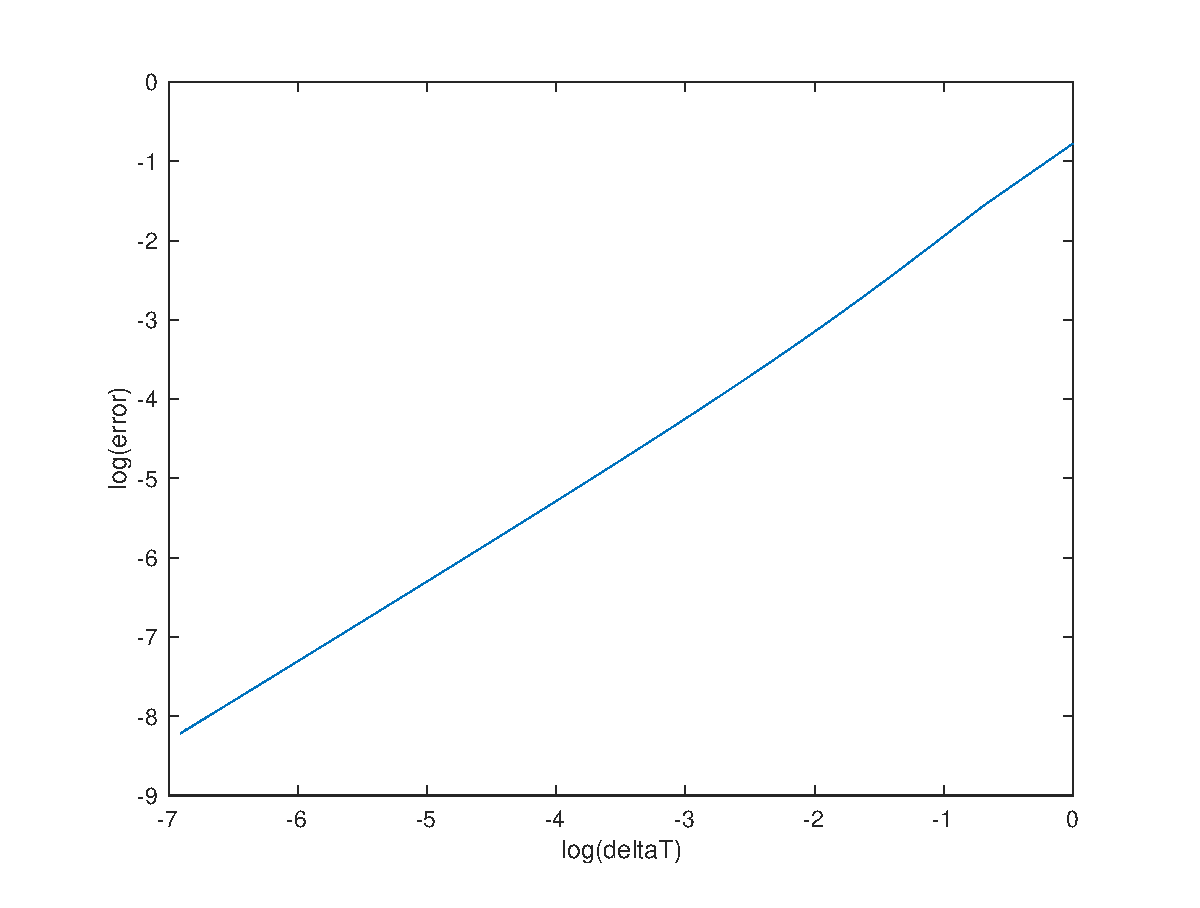
\includegraphics[width=2.2in]{euler1.eps} 
\caption{Euler method}  
\label{euler1}
\end{figure}

\begin{figure}
\begin{minipage}[t]{0.5\textwidth}
\centering
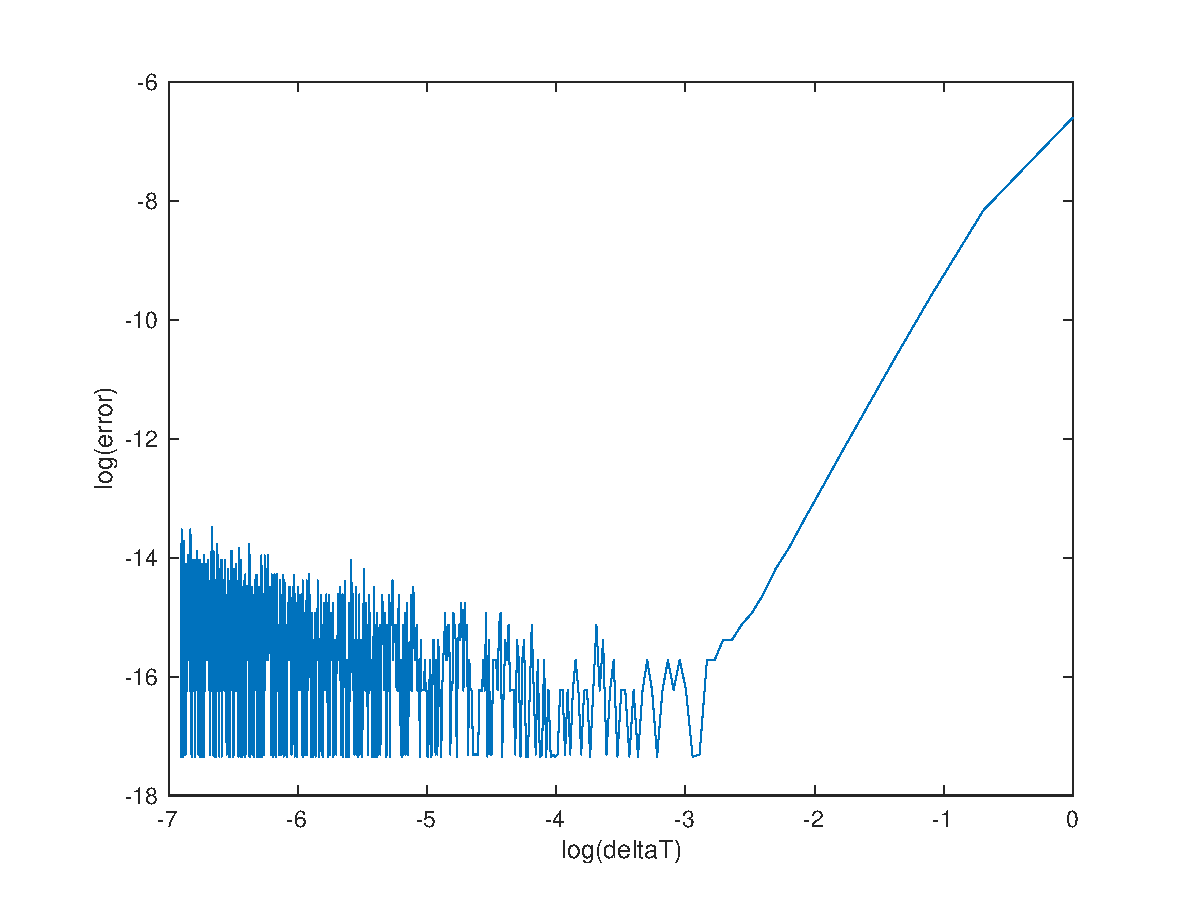
\includegraphics[width=2.2in]{leapfrog1.eps}
\caption{leapfrog method}
\label{leapfrog1}
\end{minipage}%
\begin{minipage}[t]{0.5\textwidth}
\centering
\includegraphics[width=2.2in]{rk1.eps}
\caption{Runge-Kutta method}
\label{rk1}
\end{minipage}
\end{figure}
\newpage

\section{Task 2}
In this task, we set the total time(duration) to 1000 and time step to 0.01(using smaller number the error would be smaller too, but would slow down the computer).\\
The picture \ref{euler2} shown below is the result of Euler method.
\\
The picture \ref{leapfrog2} shown below is the result of Leapfrog method.
\\
The picture \ref{rk2} shown below is the result of Runge-Kutta method.
\\
AS the result shown in these pictures, we can see that when the time step is same, the Runge-Kutta method(which error is about \({10^{ - 5}}\)) is better then Leapfrog method(which error is about \({10^{ - 3}}\)); and the Leapfrog method is better then Euler method(which error is about \({10^{2}}\)).

\begin{figure}  
\centering  
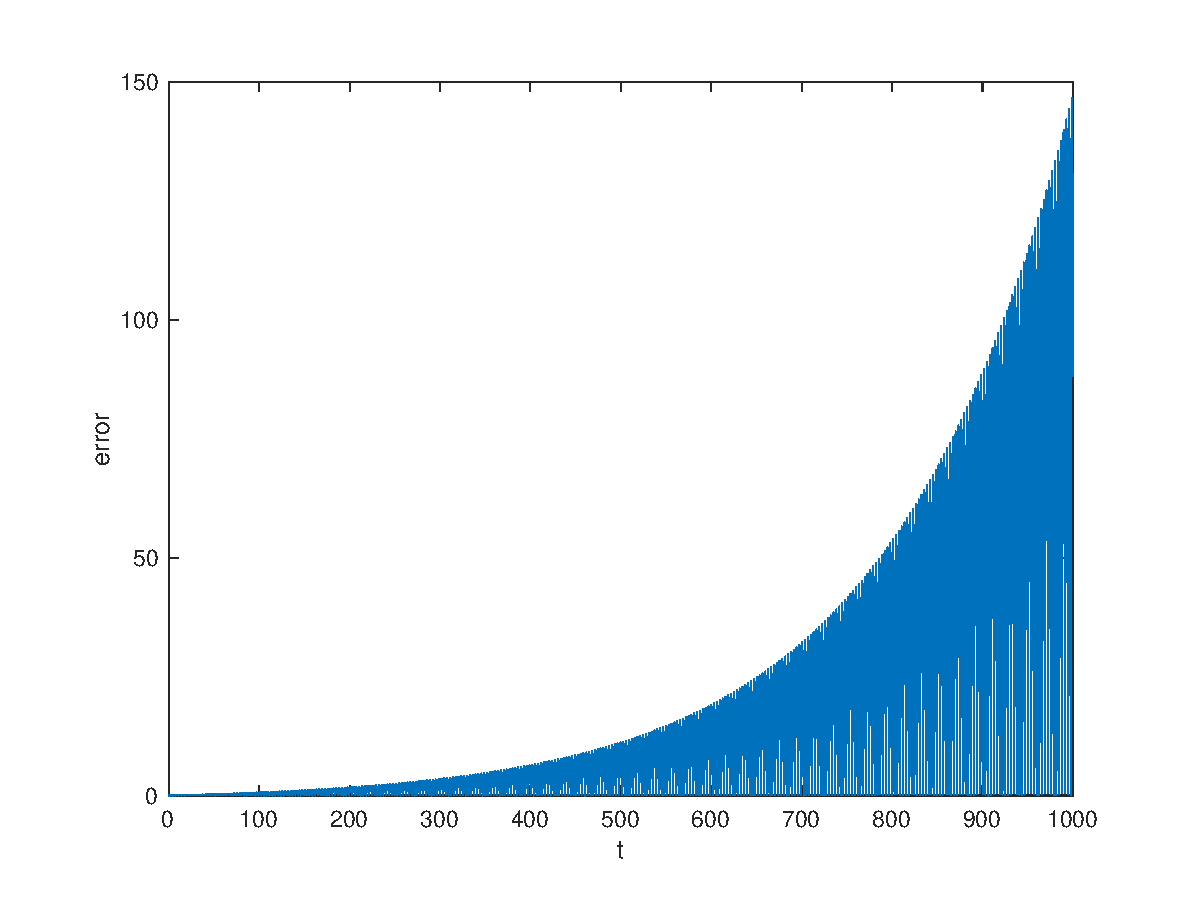
\includegraphics[width=2.2in]{euler2.eps} 
\caption{Euler method}  
\label{euler2}
\end{figure}
\begin{figure}
\begin{minipage}[t]{0.5\textwidth}
\centering
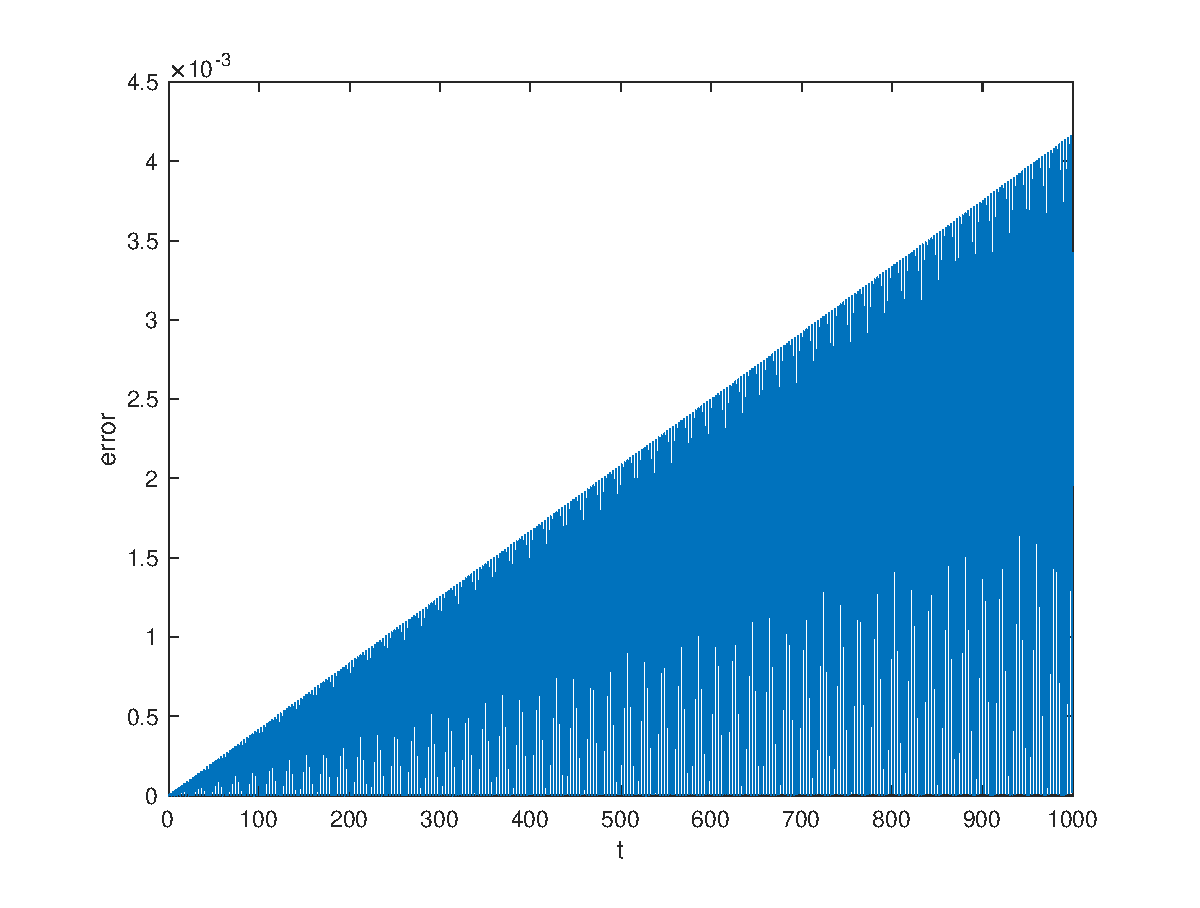
\includegraphics[width=2.2in]{leapfrog2.eps}
\caption{leapfrog method}
\label{leapfrog2}
\end{minipage}%
\begin{minipage}[t]{0.5\textwidth}
\centering
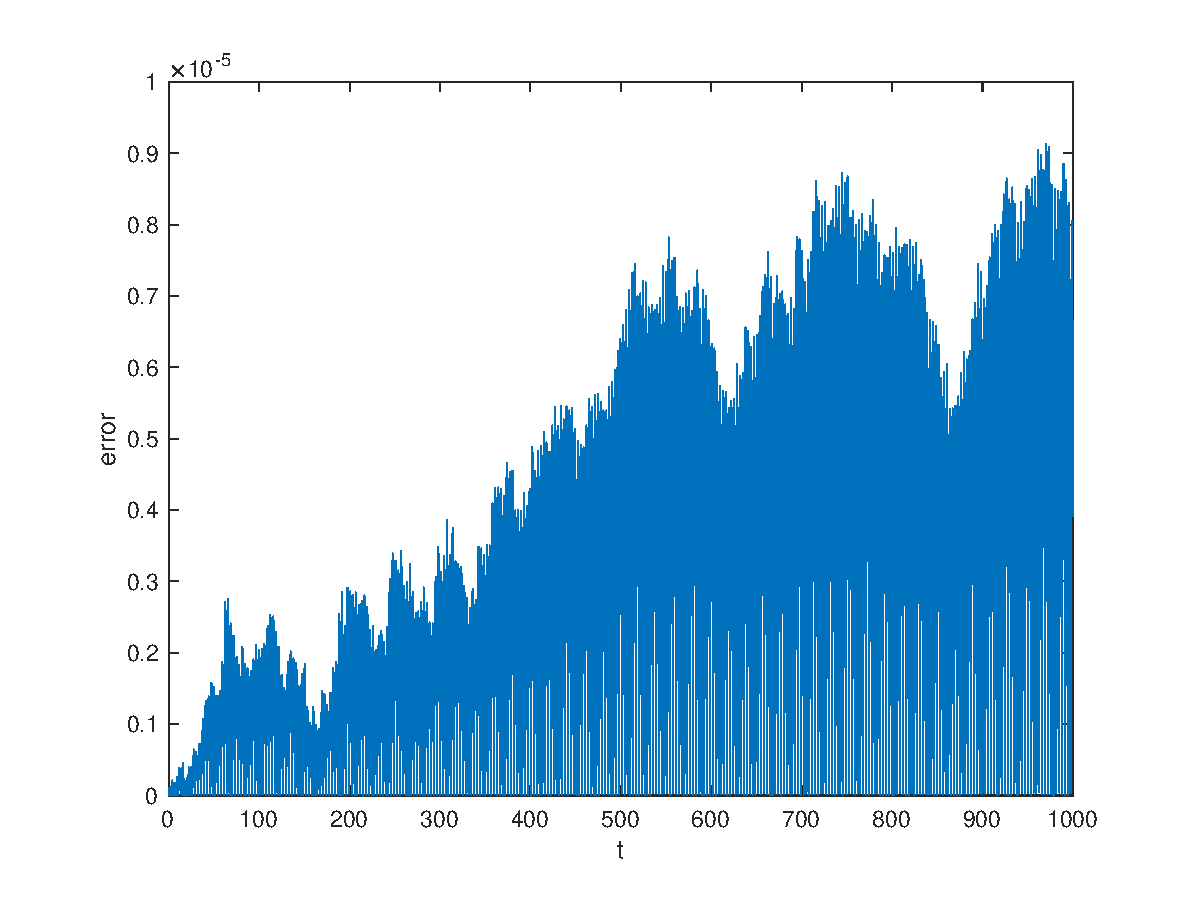
\includegraphics[width=2.2in]{rk2.eps}
\caption{Runge-Kutta method}
\label{rk2}
\end{minipage}
\end{figure}
\newpage
\section{Task 3}
In this task, we calculate the energy when using 3 different method and compare them with the real energy value(0.5). Generally, the Euler method is the worst and will violate conservation of energy by at least 100\% even when time step is 0.001. For Leapfrog method and Runge-Kutta method, we set duration to 10000000, but it runs forever so we didn't find which one is better. But from the picture, we can see that the error of Runge-Kutta keep getting larger but the error of Leapfrog method it actually come back forth from 0.5 which is the exact value of energy. so we guess that after the duration getting very large the Leapfrog method may get a better result(smaller error) then Runge-Kutta method.
\subsection{Euler method}
For Euler method, we set the duration to 1000 and time step to 3 different value of \([0.01,0.005,0.001]\).\\
The picture \ref{euler3} shown below is the result of Euler method.
\subsection{Leapfrog method}
For Euler method, we set the duration to 100000 and time step to 3 different value of \([0.01,0.005,0.001]\).
The picture \ref{leapfrog3} shown below is the result of Leapfrog method.
\subsection{Runge-Kutta method}
For Euler method, we set the duration to 100000 and time step to 3 different value of \([0.01,0.005,0.001]\).
The picture \ref{rk3} shown below is the result of Runge-Kutta method.

\begin{figure}  
\centering  
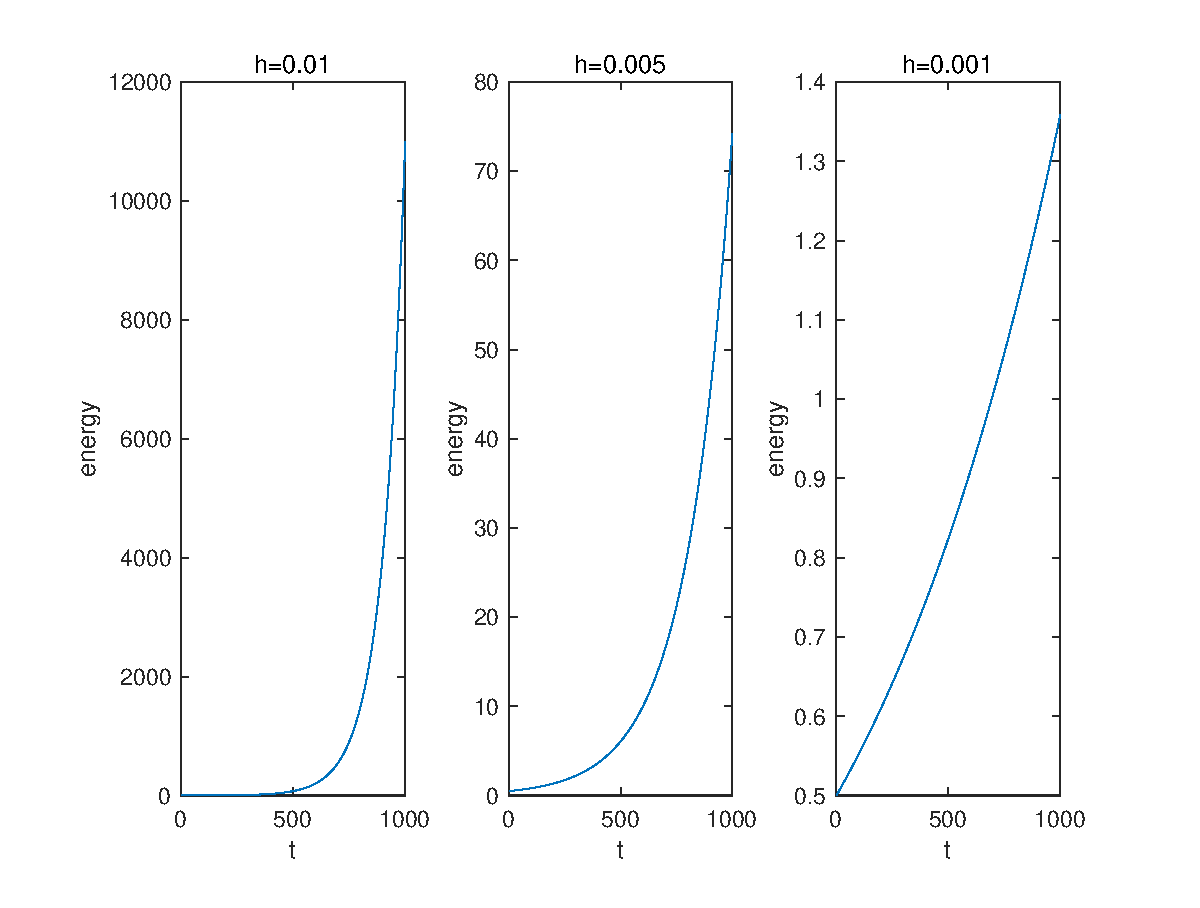
\includegraphics[scale=0.5]{euler3.eps} 
\caption{Euler method}  
\label{euler3}
\end{figure}
\begin{figure}  
\centering  
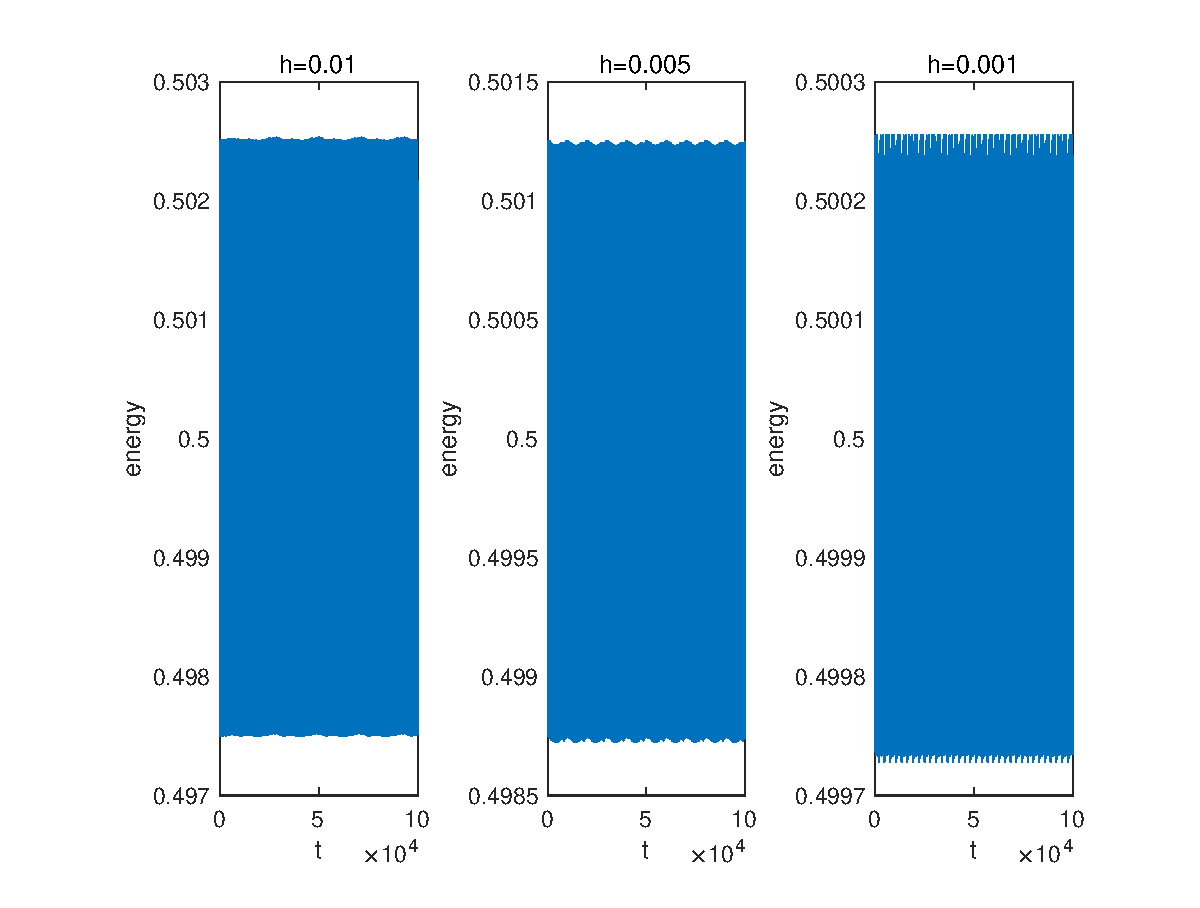
\includegraphics[scale=0.5]{leapfrog3.eps} 
\caption{leapfrog method}  
\label{leapfrog3}
\end{figure}
\begin{figure}  
\centering  
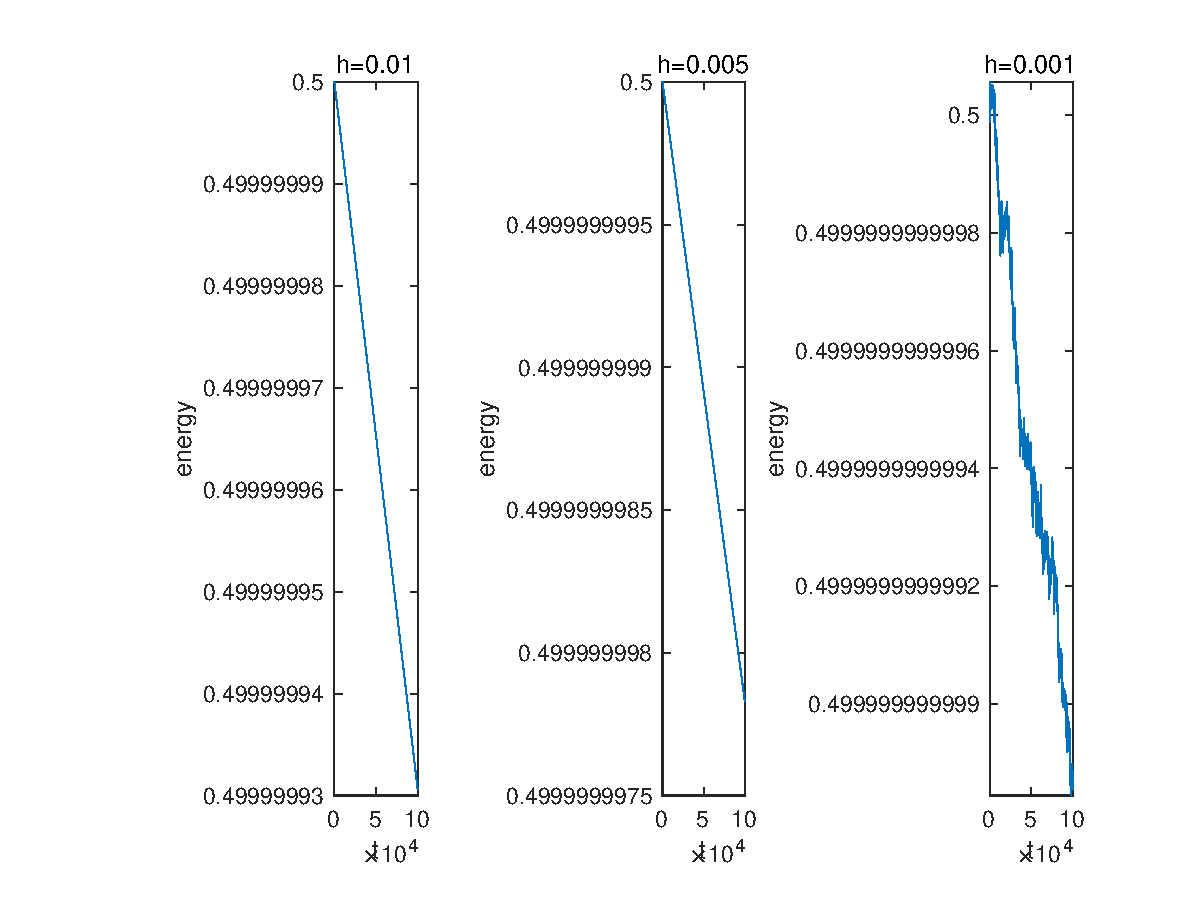
\includegraphics[scale=0.5]{rk3.eps} 
\caption{Runge-Kutta method}  
\label{rk3}
\end{figure}
 



\begin{appendices}
\section{task1 code}\label{code-1}
\subsection{Euler method}
\lstinputlisting{euler1.m}
\subsection{Leapfrog method}
\lstinputlisting{leapfrog1.m}
\subsection{Runge-Kutta method}
\lstinputlisting{rk1.m}
\section{task2 code}\label{code-2}
\subsection{Euler method}
\lstinputlisting{euler2.m}
\subsection{Leapfrog method}
\lstinputlisting{leapfrog2.m}
\subsection{Runge-Kutta method}
\lstinputlisting{rk2.m}
\section{task3 code}\label{code-3}
\subsection{Euler method}
\lstinputlisting{euler3.m}
\subsection{Leapfrog method}
\lstinputlisting{leapfrog3.m}
\subsection{Runge-Kutta method}
\lstinputlisting{rk3.m}
\subsection{Compare 3 method}
\lstinputlisting{3.m}
\end{appendices}

\end{document}